\documentclass[1p]{elsarticle_modified}
%\bibliographystyle{elsarticle-num}

%\usepackage[colorlinks]{hyperref}
%\usepackage{abbrmath_seonhwa} %\Abb, \Ascr, \Acal ,\Abf, \Afrak
\usepackage{amsfonts}
\usepackage{amssymb}
\usepackage{amsmath}
\usepackage{amsthm}
\usepackage{scalefnt}
\usepackage{amsbsy}
\usepackage{kotex}
\usepackage{caption}
\usepackage{subfig}
\usepackage{color}
\usepackage{graphicx}
\usepackage{xcolor} %% white, black, red, green, blue, cyan, magenta, yellow
\usepackage{float}
\usepackage{setspace}
\usepackage{hyperref}

\usepackage{tikz}
\usetikzlibrary{arrows}

\usepackage{multirow}
\usepackage{array} % fixed length table
\usepackage{hhline}

%%%%%%%%%%%%%%%%%%%%%
\makeatletter
\renewcommand*\env@matrix[1][\arraystretch]{%
	\edef\arraystretch{#1}%
	\hskip -\arraycolsep
	\let\@ifnextchar\new@ifnextchar
	\array{*\c@MaxMatrixCols c}}
\makeatother %https://tex.stackexchange.com/questions/14071/how-can-i-increase-the-line-spacing-in-a-matrix
%%%%%%%%%%%%%%%

\usepackage[normalem]{ulem}

\newcommand{\msout}[1]{\ifmmode\text{\sout{\ensuremath{#1}}}\else\sout{#1}\fi}
%SOURCE: \msout is \stkout macro in https://tex.stackexchange.com/questions/20609/strikeout-in-math-mode

\newcommand{\cancel}[1]{
	\ifmmode
	{\color{red}\msout{#1}}
	\else
	{\color{red}\sout{#1}}
	\fi
}

\newcommand{\add}[1]{
	{\color{blue}\uwave{#1}}
}

\newcommand{\replace}[2]{
	\ifmmode
	{\color{red}\msout{#1}}{\color{blue}\uwave{#2}}
	\else
	{\color{red}\sout{#1}}{\color{blue}\uwave{#2}}
	\fi
}

\newcommand{\Sol}{\mathcal{S}} %segment
\newcommand{\D}{D} %diagram
\newcommand{\A}{\mathcal{A}} %arc


%%%%%%%%%%%%%%%%%%%%%%%%%%%%%5 test

\def\sl{\operatorname{\textup{SL}}(2,\Cbb)}
\def\psl{\operatorname{\textup{PSL}}(2,\Cbb)}
\def\quan{\mkern 1mu \triangleright \mkern 1mu}

\theoremstyle{definition}
\newtheorem{thm}{Theorem}[section]
\newtheorem{prop}[thm]{Proposition}
\newtheorem{lem}[thm]{Lemma}
\newtheorem{ques}[thm]{Question}
\newtheorem{cor}[thm]{Corollary}
\newtheorem{defn}[thm]{Definition}
\newtheorem{exam}[thm]{Example}
\newtheorem{rmk}[thm]{Remark}
\newtheorem{alg}[thm]{Algorithm}

\newcommand{\I}{\sqrt{-1}}
\begin{document}

%\begin{frontmatter}
%
%\title{Boundary parabolic representations of knots up to 8 crossings}
%
%%% Group authors per affiliation:
%\author{Yunhi Cho} 
%\address{Department of Mathematics, University of Seoul, Seoul, Korea}
%\ead{yhcho@uos.ac.kr}
%
%
%\author{Seonhwa Kim} %\fnref{s_kim}}
%\address{Center for Geometry and Physics, Institute for Basic Science, Pohang, 37673, Korea}
%\ead{ryeona17@ibs.re.kr}
%
%\author{Hyuk Kim}
%\address{Department of Mathematical Sciences, Seoul National University, Seoul 08826, Korea}
%\ead{hyukkim@snu.ac.kr}
%
%\author{Seokbeom Yoon}
%\address{Department of Mathematical Sciences, Seoul National University, Seoul, 08826,  Korea}
%\ead{sbyoon15@snu.ac.kr}
%
%\begin{abstract}
%We find all boundary parabolic representation of knots up to 8 crossings.
%
%\end{abstract}
%\begin{keyword}
%    \MSC[2010] 57M25 
%\end{keyword}
%
%\end{frontmatter}

%\linenumbers
%\tableofcontents
%
\newcommand\colored[1]{\textcolor{white}{\rule[-0.35ex]{0.8em}{1.4ex}}\kern-0.8em\color{red} #1}%
%\newcommand\colored[1]{\textcolor{white}{ #1}\kern-2.17ex	\textcolor{white}{ #1}\kern-1.81ex	\textcolor{white}{ #1}\kern-2.15ex\color{red}#1	}

{\Large $\underline{12a_{0524}~(K12a_{0524})}$}

\setlength{\tabcolsep}{10pt}
\renewcommand{\arraystretch}{1.6}
\vspace{1cm}\begin{tabular}{m{100pt}>{\centering\arraybackslash}m{274pt}}
\multirow{5}{120pt}{
	\centering
	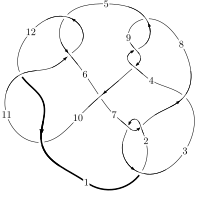
\includegraphics[width=112pt]{../../../GIT/diagram.site/Diagrams/png/1325_12a_0524.png}\\
\ \ \ A knot diagram\footnotemark}&
\allowdisplaybreaks
\textbf{Linearized knot diagam} \\
\cline{2-2}
 &
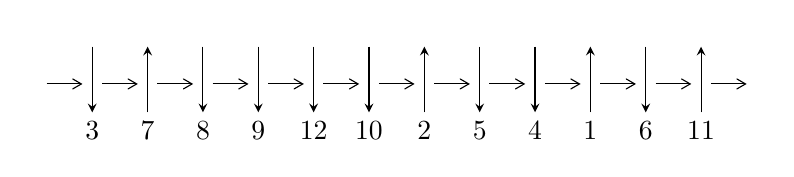
\begin{tikzpicture}[x=20pt, y=17pt]
	% nodes
	\node (C0) at (0, 0) {};
	\node (C1) at (1, 0) {};
	\node (C1U) at (1, +1) {};
	\node (C1D) at (1, -1) {3};

	\node (C2) at (2, 0) {};
	\node (C2U) at (2, +1) {};
	\node (C2D) at (2, -1) {7};

	\node (C3) at (3, 0) {};
	\node (C3U) at (3, +1) {};
	\node (C3D) at (3, -1) {8};

	\node (C4) at (4, 0) {};
	\node (C4U) at (4, +1) {};
	\node (C4D) at (4, -1) {9};

	\node (C5) at (5, 0) {};
	\node (C5U) at (5, +1) {};
	\node (C5D) at (5, -1) {12};

	\node (C6) at (6, 0) {};
	\node (C6U) at (6, +1) {};
	\node (C6D) at (6, -1) {10};

	\node (C7) at (7, 0) {};
	\node (C7U) at (7, +1) {};
	\node (C7D) at (7, -1) {2};

	\node (C8) at (8, 0) {};
	\node (C8U) at (8, +1) {};
	\node (C8D) at (8, -1) {5};

	\node (C9) at (9, 0) {};
	\node (C9U) at (9, +1) {};
	\node (C9D) at (9, -1) {4};

	\node (C10) at (10, 0) {};
	\node (C10U) at (10, +1) {};
	\node (C10D) at (10, -1) {1};

	\node (C11) at (11, 0) {};
	\node (C11U) at (11, +1) {};
	\node (C11D) at (11, -1) {6};

	\node (C12) at (12, 0) {};
	\node (C12U) at (12, +1) {};
	\node (C12D) at (12, -1) {11};
	\node (C13) at (13, 0) {};

	% arrows
	\draw[->,>={angle 60}]
	(C0) edge (C1) (C1) edge (C2) (C2) edge (C3) (C3) edge (C4) (C4) edge (C5) (C5) edge (C6) (C6) edge (C7) (C7) edge (C8) (C8) edge (C9) (C9) edge (C10) (C10) edge (C11) (C11) edge (C12) (C12) edge (C13) ;	\draw[->,>=stealth]
	(C1U) edge (C1D) (C2D) edge (C2U) (C3U) edge (C3D) (C4U) edge (C4D) (C5U) edge (C5D) (C6U) edge (C6D) (C7D) edge (C7U) (C8U) edge (C8D) (C9U) edge (C9D) (C10D) edge (C10U) (C11U) edge (C11D) (C12D) edge (C12U) ;
	\end{tikzpicture} \\
\hhline{~~} \\& 
\textbf{Solving Sequence} \\ \cline{2-2} 
 &
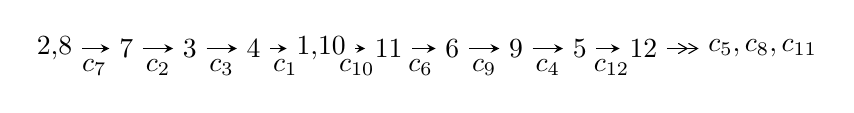
\begin{tikzpicture}[x=23pt, y=7pt]
	% node
	\node (A0) at (-1/8, 0) {2,8};
	\node (A1) at (1, 0) {7};
	\node (A2) at (2, 0) {3};
	\node (A3) at (3, 0) {4};
	\node (A4) at (65/16, 0) {1,10};
	\node (A5) at (41/8, 0) {11};
	\node (A6) at (49/8, 0) {6};
	\node (A7) at (57/8, 0) {9};
	\node (A8) at (65/8, 0) {5};
	\node (A9) at (73/8, 0) {12};
	\node (C1) at (1/2, -1) {$c_{7}$};
	\node (C2) at (3/2, -1) {$c_{2}$};
	\node (C3) at (5/2, -1) {$c_{3}$};
	\node (C4) at (7/2, -1) {$c_{1}$};
	\node (C5) at (37/8, -1) {$c_{10}$};
	\node (C6) at (45/8, -1) {$c_{6}$};
	\node (C7) at (53/8, -1) {$c_{9}$};
	\node (C8) at (61/8, -1) {$c_{4}$};
	\node (C9) at (69/8, -1) {$c_{12}$};
	\node (A10) at (11, 0) {$c_{5},c_{8},c_{11}$};

	% edge
	\draw[->,>=stealth]	
	(A0) edge (A1) (A1) edge (A2) (A2) edge (A3) (A3) edge (A4) (A4) edge (A5) (A5) edge (A6) (A6) edge (A7) (A7) edge (A8) (A8) edge (A9) ;
	\draw[->>,>={angle 60}]	
	(A9) edge (A10);
\end{tikzpicture} \\ 

\end{tabular} \\

\footnotetext{
The image of knot diagram is generated by the software ``\textbf{Draw programme}" developed by Andrew Bartholomew(\url{http://www.layer8.co.uk/maths/draw/index.htm\#Running-draw}), where we modified some parts for our purpose(\url{https://github.com/CATsTAILs/LinksPainter}).
}\phantom \\ \newline 
\centering \textbf{Ideals for irreducible components\footnotemark of $X_{\text{par}}$} 
 
\begin{align*}
I^u_{1}&=\langle 
1.19165\times10^{29} u^{63}+7.17172\times10^{28} u^{62}+\cdots+8.78717\times10^{29} b+1.18770\times10^{30},\\
\phantom{I^u_{1}}&\phantom{= \langle  }1.42661\times10^{31} u^{63}-8.31260\times10^{30} u^{62}+\cdots+7.02973\times10^{30} a+1.31917\times10^{31},\;u^{64}- u^{63}+\cdots-2 u+1\rangle \\
I^u_{2}&=\langle 
- u^4-2 u^2+b,\;u^4+u^2+a-1,\;u^{27}+9 u^{25}+\cdots- u-1\rangle \\
I^u_{3}&=\langle 
b+1,\;a^3- a^2 u-3 a^2+2 a u+a+1,\;u^2+1\rangle \\
\\
\end{align*}
\raggedright * 3 irreducible components of $\dim_{\mathbb{C}}=0$, with total 97 representations.\\
\footnotetext{All coefficients of polynomials are rational numbers. But the coefficients are sometimes approximated in decimal forms when there is not enough margin.}
\newpage
\renewcommand{\arraystretch}{1}
\centering \section*{I. $I^u_{1}= \langle 1.19\times10^{29} u^{63}+7.17\times10^{28} u^{62}+\cdots+8.79\times10^{29} b+1.19\times10^{30},\;1.43\times10^{31} u^{63}-8.31\times10^{30} u^{62}+\cdots+7.03\times10^{30} a+1.32\times10^{31},\;u^{64}- u^{63}+\cdots-2 u+1 \rangle$}
\flushleft \textbf{(i) Arc colorings}\\
\begin{tabular}{m{7pt} m{180pt} m{7pt} m{180pt} }
\flushright $a_{2}=$&$\begin{pmatrix}0\\u\end{pmatrix}$ \\
\flushright $a_{8}=$&$\begin{pmatrix}1\\0\end{pmatrix}$ \\
\flushright $a_{7}=$&$\begin{pmatrix}1\\u^2\end{pmatrix}$ \\
\flushright $a_{3}=$&$\begin{pmatrix}u\\u^3+u\end{pmatrix}$ \\
\flushright $a_{4}=$&$\begin{pmatrix}- u^3\\u^3+u\end{pmatrix}$ \\
\flushright $a_{1}=$&$\begin{pmatrix}u^3\\u^5+u^3+u\end{pmatrix}$ \\
\flushright $a_{10}=$&$\begin{pmatrix}-2.02940 u^{63}+1.18249 u^{62}+\cdots-2.99982 u-1.87655\\-0.135612 u^{63}-0.0816158 u^{62}+\cdots+0.389219 u-1.35163\end{pmatrix}$ \\
\flushright $a_{11}=$&$\begin{pmatrix}-2.09643 u^{63}+1.12088 u^{62}+\cdots-3.17116 u-1.64675\\-0.314315 u^{63}-0.0337323 u^{62}+\cdots-0.348072 u-1.64704\end{pmatrix}$ \\
\flushright $a_{6}=$&$\begin{pmatrix}-1.85442 u^{63}+0.738976 u^{62}+\cdots-1.32676 u-3.25750\\-0.355484 u^{63}+0.0412247 u^{62}+\cdots-0.0480554 u-2.11408\end{pmatrix}$ \\
\flushright $a_{9}=$&$\begin{pmatrix}-2.16501 u^{63}+1.10088 u^{62}+\cdots-2.61060 u-2.22819\\-0.314049 u^{63}-0.0375849 u^{62}+\cdots-0.543961 u-1.53479\end{pmatrix}$ \\
\flushright $a_{5}=$&$\begin{pmatrix}-2.41577 u^{63}+2.96723 u^{62}+\cdots-13.7211 u+4.47906\\-0.534793 u^{63}+0.848842 u^{62}+\cdots-4.03951 u+1.61355\end{pmatrix}$ \\
\flushright $a_{12}=$&$\begin{pmatrix}-2.57675 u^{63}+2.92049 u^{62}+\cdots-15.0731 u+4.77964\\-0.807524 u^{63}+1.17773 u^{62}+\cdots-5.99028 u+1.80950\end{pmatrix}$\\&\end{tabular}
\flushleft \textbf{(ii) Obstruction class $= -1$}\\~\\
\flushleft \textbf{(iii) Cusp Shapes $= -2.60252 u^{63}+1.80827 u^{62}+\cdots-15.4271 u+3.07685$}\\~\\
\newpage\renewcommand{\arraystretch}{1}
\flushleft \textbf{(iv) u-Polynomials at the component}\newline \\
\begin{tabular}{m{50pt}|m{274pt}}
Crossings & \hspace{64pt}u-Polynomials at each crossing \\
\hline $$\begin{aligned}c_{1}\end{aligned}$$&$\begin{aligned}
&u^{64}+31 u^{63}+\cdots+8 u+1
\end{aligned}$\\
\hline $$\begin{aligned}c_{2},c_{7}\end{aligned}$$&$\begin{aligned}
&u^{64}+u^{63}+\cdots+2 u+1
\end{aligned}$\\
\hline $$\begin{aligned}c_{3}\end{aligned}$$&$\begin{aligned}
&u^{64}+2 u^{63}+\cdots+1984 u+128
\end{aligned}$\\
\hline $$\begin{aligned}c_{4},c_{8},c_{9}\end{aligned}$$&$\begin{aligned}
&u^{64}+u^{63}+\cdots+16 u+1
\end{aligned}$\\
\hline $$\begin{aligned}c_{5},c_{11}\end{aligned}$$&$\begin{aligned}
&u^{64}+2 u^{63}+\cdots+u+2
\end{aligned}$\\
\hline $$\begin{aligned}c_{6}\end{aligned}$$&$\begin{aligned}
&u^{64}-10 u^{63}+\cdots-14873 u+1862
\end{aligned}$\\
\hline $$\begin{aligned}c_{10},c_{12}\end{aligned}$$&$\begin{aligned}
&u^{64}-20 u^{63}+\cdots-19 u+4
\end{aligned}$\\
\hline
\end{tabular}\\~\\
\newpage\renewcommand{\arraystretch}{1}
\flushleft \textbf{(v) Riley Polynomials at the component}\newline \\
\begin{tabular}{m{50pt}|m{274pt}}
Crossings & \hspace{64pt}Riley Polynomials at each crossing \\
\hline $$\begin{aligned}c_{1}\end{aligned}$$&$\begin{aligned}
&y^{64}+11 y^{63}+\cdots-40 y+1
\end{aligned}$\\
\hline $$\begin{aligned}c_{2},c_{7}\end{aligned}$$&$\begin{aligned}
&y^{64}+31 y^{63}+\cdots+8 y+1
\end{aligned}$\\
\hline $$\begin{aligned}c_{3}\end{aligned}$$&$\begin{aligned}
&y^{64}-30 y^{63}+\cdots+1945600 y+16384
\end{aligned}$\\
\hline $$\begin{aligned}c_{4},c_{8},c_{9}\end{aligned}$$&$\begin{aligned}
&y^{64}+59 y^{63}+\cdots+104 y+1
\end{aligned}$\\
\hline $$\begin{aligned}c_{5},c_{11}\end{aligned}$$&$\begin{aligned}
&y^{64}+20 y^{63}+\cdots+19 y+4
\end{aligned}$\\
\hline $$\begin{aligned}c_{6}\end{aligned}$$&$\begin{aligned}
&y^{64}-12 y^{63}+\cdots-37020813 y+3467044
\end{aligned}$\\
\hline $$\begin{aligned}c_{10},c_{12}\end{aligned}$$&$\begin{aligned}
&y^{64}+48 y^{63}+\cdots+879 y+16
\end{aligned}$\\
\hline
\end{tabular}\\~\\
\newpage\flushleft \textbf{(vi) Complex Volumes and Cusp Shapes}
$$\begin{array}{c|c|c}  
\text{Solutions to }I^u_{1}& \I (\text{vol} + \sqrt{-1}CS) & \text{Cusp shape}\\
 \hline 
\begin{aligned}
u &= -0.740864 + 0.662784 I \\
a &= -1.076250 + 0.014411 I \\
b &= \phantom{-}0.049744 + 0.197245 I\end{aligned}
 & \phantom{-}6.16267 + 3.38539 I & \phantom{-}2.09489 - 2.71260 I \\ \hline\begin{aligned}
u &= -0.740864 - 0.662784 I \\
a &= -1.076250 - 0.014411 I \\
b &= \phantom{-}0.049744 - 0.197245 I\end{aligned}
 & \phantom{-}6.16267 - 3.38539 I & \phantom{-}2.09489 + 2.71260 I \\ \hline\begin{aligned}
u &= -0.445418 + 0.865420 I \\
a &= -0.339938 - 0.644967 I \\
b &= \phantom{-}0.121992 + 1.067110 I\end{aligned}
 & -1.53101 - 1.39020 I & -5.91926 + 3.88104 I \\ \hline\begin{aligned}
u &= -0.445418 - 0.865420 I \\
a &= -0.339938 + 0.644967 I \\
b &= \phantom{-}0.121992 - 1.067110 I\end{aligned}
 & -1.53101 + 1.39020 I & -5.91926 - 3.88104 I \\ \hline\begin{aligned}
u &= -0.021735 + 1.036710 I \\
a &= \phantom{-}1.165230 + 0.128138 I \\
b &= -0.0067591 - 0.0148508 I\end{aligned}
 & -4.65557 - 2.80220 I & -13.46250 + 3.05850 I \\ \hline\begin{aligned}
u &= -0.021735 - 1.036710 I \\
a &= \phantom{-}1.165230 - 0.128138 I \\
b &= -0.0067591 + 0.0148508 I\end{aligned}
 & -4.65557 + 2.80220 I & -13.46250 - 3.05850 I \\ \hline\begin{aligned}
u &= \phantom{-}0.510043 + 0.798911 I \\
a &= -0.241579 + 1.067010 I \\
b &= -0.181458 - 1.313360 I\end{aligned}
 & -0.86573 + 6.45035 I & -3.51752 - 9.65683 I \\ \hline\begin{aligned}
u &= \phantom{-}0.510043 - 0.798911 I \\
a &= -0.241579 - 1.067010 I \\
b &= -0.181458 + 1.313360 I\end{aligned}
 & -0.86573 - 6.45035 I & -3.51752 + 9.65683 I \\ \hline\begin{aligned}
u &= -0.715186 + 0.790541 I \\
a &= -0.816990 + 0.099941 I \\
b &= \phantom{-}0.096344 - 0.304633 I\end{aligned}
 & \phantom{-}9.65441 - 2.68529 I & \phantom{-}5.74999 + 0. I\phantom{ +0.000000I} \\ \hline\begin{aligned}
u &= -0.715186 - 0.790541 I \\
a &= -0.816990 - 0.099941 I \\
b &= \phantom{-}0.096344 + 0.304633 I\end{aligned}
 & \phantom{-}9.65441 + 2.68529 I & \phantom{-}5.74999 + 0. I\phantom{ +0.000000I}\\
 \hline 
 \end{array}$$\newpage$$\begin{array}{c|c|c}  
\text{Solutions to }I^u_{1}& \I (\text{vol} + \sqrt{-1}CS) & \text{Cusp shape}\\
 \hline 
\begin{aligned}
u &= \phantom{-}0.636482 + 0.681496 I \\
a &= -1.048850 + 0.124326 I \\
b &= -0.239480 - 0.007765 I\end{aligned}
 & \phantom{-}4.80153 + 1.37625 I & -0.64369 - 3.25078 I \\ \hline\begin{aligned}
u &= \phantom{-}0.636482 - 0.681496 I \\
a &= -1.048850 - 0.124326 I \\
b &= -0.239480 + 0.007765 I\end{aligned}
 & \phantom{-}4.80153 - 1.37625 I & -0.64369 + 3.25078 I \\ \hline\begin{aligned}
u &= \phantom{-}0.897043 + 0.224964 I \\
a &= -0.162901 + 0.141407 I \\
b &= -1.21809 - 1.38009 I\end{aligned}
 & \phantom{-}1.29409 - 11.08640 I & -1.19961 + 7.21378 I \\ \hline\begin{aligned}
u &= \phantom{-}0.897043 - 0.224964 I \\
a &= -0.162901 - 0.141407 I \\
b &= -1.21809 + 1.38009 I\end{aligned}
 & \phantom{-}1.29409 + 11.08640 I & -1.19961 - 7.21378 I \\ \hline\begin{aligned}
u &= \phantom{-}0.631106 + 0.872776 I \\
a &= -0.402460 + 0.142378 I \\
b &= -0.248913 + 0.600652 I\end{aligned}
 & \phantom{-}4.24624 + 3.53311 I & \phantom{-0.000000 } 0 \\ \hline\begin{aligned}
u &= \phantom{-}0.631106 - 0.872776 I \\
a &= -0.402460 - 0.142378 I \\
b &= -0.248913 - 0.600652 I\end{aligned}
 & \phantom{-}4.24624 - 3.53311 I & \phantom{-0.000000 } 0 \\ \hline\begin{aligned}
u &= \phantom{-}0.846306 + 0.300514 I \\
a &= -0.501209 + 0.065356 I \\
b &= -0.87761 - 1.19110 I\end{aligned}
 & \phantom{-}6.84859 - 5.40917 I & \phantom{-}4.32977 + 4.44506 I \\ \hline\begin{aligned}
u &= \phantom{-}0.846306 - 0.300514 I \\
a &= -0.501209 - 0.065356 I \\
b &= -0.87761 + 1.19110 I\end{aligned}
 & \phantom{-}6.84859 + 5.40917 I & \phantom{-}4.32977 - 4.44506 I \\ \hline\begin{aligned}
u &= -0.871978 + 0.210846 I \\
a &= -0.151648 - 0.024372 I \\
b &= -1.25701 + 1.25917 I\end{aligned}
 & \phantom{-}0.32985 + 5.28991 I & -2.86725 - 2.43047 I \\ \hline\begin{aligned}
u &= -0.871978 - 0.210846 I \\
a &= -0.151648 + 0.024372 I \\
b &= -1.25701 - 1.25917 I\end{aligned}
 & \phantom{-}0.32985 - 5.28991 I & -2.86725 + 2.43047 I\\
 \hline 
 \end{array}$$\newpage$$\begin{array}{c|c|c}  
\text{Solutions to }I^u_{1}& \I (\text{vol} + \sqrt{-1}CS) & \text{Cusp shape}\\
 \hline 
\begin{aligned}
u &= -0.687105 + 0.897262 I \\
a &= -0.355479 + 0.167421 I \\
b &= -0.048600 - 0.750276 I\end{aligned}
 & \phantom{-}5.48639 - 8.73923 I & \phantom{-0.000000 } 0 \\ \hline\begin{aligned}
u &= -0.687105 - 0.897262 I \\
a &= -0.355479 - 0.167421 I \\
b &= -0.048600 + 0.750276 I\end{aligned}
 & \phantom{-}5.48639 + 8.73923 I & \phantom{-0.000000 } 0 \\ \hline\begin{aligned}
u &= -0.373591 + 1.075490 I \\
a &= -0.795520 + 0.588147 I \\
b &= \phantom{-}0.914345 + 0.454271 I\end{aligned}
 & -1.62900 - 0.89969 I & \phantom{-0.000000 } 0 \\ \hline\begin{aligned}
u &= -0.373591 - 1.075490 I \\
a &= -0.795520 - 0.588147 I \\
b &= \phantom{-}0.914345 - 0.454271 I\end{aligned}
 & -1.62900 + 0.89969 I & \phantom{-0.000000 } 0 \\ \hline\begin{aligned}
u &= \phantom{-}0.731325 + 0.421281 I \\
a &= -0.938294 - 0.092021 I \\
b &= -0.543242 - 0.716970 I\end{aligned}
 & \phantom{-}5.06057 + 0.57857 I & \phantom{-}2.53258 - 2.78290 I \\ \hline\begin{aligned}
u &= \phantom{-}0.731325 - 0.421281 I \\
a &= -0.938294 + 0.092021 I \\
b &= -0.543242 + 0.716970 I\end{aligned}
 & \phantom{-}5.06057 - 0.57857 I & \phantom{-}2.53258 + 2.78290 I \\ \hline\begin{aligned}
u &= \phantom{-}0.434112 + 1.098840 I \\
a &= \phantom{-}1.43799 + 1.59048 I \\
b &= -1.29963 + 0.70752 I\end{aligned}
 & -3.91899 + 0.31574 I & \phantom{-0.000000 } 0 \\ \hline\begin{aligned}
u &= \phantom{-}0.434112 - 1.098840 I \\
a &= \phantom{-}1.43799 - 1.59048 I \\
b &= -1.29963 - 0.70752 I\end{aligned}
 & -3.91899 - 0.31574 I & \phantom{-0.000000 } 0 \\ \hline\begin{aligned}
u &= -0.176032 + 0.776472 I \\
a &= \phantom{-}0.607805 - 0.218610 I \\
b &= -0.208597 + 0.304278 I\end{aligned}
 & -0.537446 - 1.039780 I & -7.39933 + 6.43993 I \\ \hline\begin{aligned}
u &= -0.176032 - 0.776472 I \\
a &= \phantom{-}0.607805 + 0.218610 I \\
b &= -0.208597 - 0.304278 I\end{aligned}
 & -0.537446 + 1.039780 I & -7.39933 - 6.43993 I\\
 \hline 
 \end{array}$$\newpage$$\begin{array}{c|c|c}  
\text{Solutions to }I^u_{1}& \I (\text{vol} + \sqrt{-1}CS) & \text{Cusp shape}\\
 \hline 
\begin{aligned}
u &= -0.449003 + 1.119080 I \\
a &= \phantom{-}1.63202 - 1.42381 I \\
b &= -1.36040 - 0.78973 I\end{aligned}
 & -4.40703 - 6.33923 I & \phantom{-0.000000 } 0 \\ \hline\begin{aligned}
u &= -0.449003 - 1.119080 I \\
a &= \phantom{-}1.63202 + 1.42381 I \\
b &= -1.36040 + 0.78973 I\end{aligned}
 & -4.40703 + 6.33923 I & \phantom{-0.000000 } 0 \\ \hline\begin{aligned}
u &= -0.744106 + 0.270463 I \\
a &= -0.563605 + 0.288717 I \\
b &= -0.979045 + 0.832531 I\end{aligned}
 & \phantom{-}2.95946 + 3.06631 I & -2.59881 - 2.85106 I \\ \hline\begin{aligned}
u &= -0.744106 - 0.270463 I \\
a &= -0.563605 - 0.288717 I \\
b &= -0.979045 - 0.832531 I\end{aligned}
 & \phantom{-}2.95946 - 3.06631 I & -2.59881 + 2.85106 I \\ \hline\begin{aligned}
u &= \phantom{-}0.552939 + 1.084820 I \\
a &= \phantom{-}1.189260 + 0.464726 I \\
b &= -1.00752 + 1.13246 I\end{aligned}
 & \phantom{-}3.08597 + 4.29718 I & \phantom{-0.000000 } 0 \\ \hline\begin{aligned}
u &= \phantom{-}0.552939 - 1.084820 I \\
a &= \phantom{-}1.189260 - 0.464726 I \\
b &= -1.00752 - 1.13246 I\end{aligned}
 & \phantom{-}3.08597 - 4.29718 I & \phantom{-0.000000 } 0 \\ \hline\begin{aligned}
u &= \phantom{-}0.446332 + 1.136180 I \\
a &= -1.55976 - 0.67921 I \\
b &= \phantom{-}1.45534 - 0.61315 I\end{aligned}
 & -4.21610 + 3.94313 I & \phantom{-0.000000 } 0 \\ \hline\begin{aligned}
u &= \phantom{-}0.446332 - 1.136180 I \\
a &= -1.55976 + 0.67921 I \\
b &= \phantom{-}1.45534 + 0.61315 I\end{aligned}
 & -4.21610 - 3.94313 I & \phantom{-0.000000 } 0 \\ \hline\begin{aligned}
u &= -0.503355 + 1.117530 I \\
a &= -1.83906 + 0.22387 I \\
b &= \phantom{-}1.52918 + 1.02332 I\end{aligned}
 & -0.69715 - 6.51856 I & \phantom{-0.000000 } 0 \\ \hline\begin{aligned}
u &= -0.503355 - 1.117530 I \\
a &= -1.83906 - 0.22387 I \\
b &= \phantom{-}1.52918 - 1.02332 I\end{aligned}
 & -0.69715 + 6.51856 I & \phantom{-0.000000 } 0\\
 \hline 
 \end{array}$$\newpage$$\begin{array}{c|c|c}  
\text{Solutions to }I^u_{1}& \I (\text{vol} + \sqrt{-1}CS) & \text{Cusp shape}\\
 \hline 
\begin{aligned}
u &= -0.351656 + 1.195310 I \\
a &= -1.06860 + 1.58590 I \\
b &= \phantom{-}1.336950 - 0.118755 I\end{aligned}
 & -7.69997 + 3.36567 I & \phantom{-0.000000 } 0 \\ \hline\begin{aligned}
u &= -0.351656 - 1.195310 I \\
a &= -1.06860 - 1.58590 I \\
b &= \phantom{-}1.336950 + 0.118755 I\end{aligned}
 & -7.69997 - 3.36567 I & \phantom{-0.000000 } 0 \\ \hline\begin{aligned}
u &= \phantom{-}0.433087 + 0.616507 I \\
a &= \phantom{-}0.476384 + 1.128510 I \\
b &= -0.703167 - 0.846414 I\end{aligned}
 & \phantom{-}2.94099 + 1.46804 I & \phantom{-}3.65440 - 4.55346 I \\ \hline\begin{aligned}
u &= \phantom{-}0.433087 - 0.616507 I \\
a &= \phantom{-}0.476384 - 1.128510 I \\
b &= -0.703167 + 0.846414 I\end{aligned}
 & \phantom{-}2.94099 - 1.46804 I & \phantom{-}3.65440 + 4.55346 I \\ \hline\begin{aligned}
u &= \phantom{-}0.373707 + 1.194340 I \\
a &= -1.25946 - 1.48885 I \\
b &= \phantom{-}1.44389 + 0.01555 I\end{aligned}
 & -8.31434 + 2.51326 I & \phantom{-0.000000 } 0 \\ \hline\begin{aligned}
u &= \phantom{-}0.373707 - 1.194340 I \\
a &= -1.25946 + 1.48885 I \\
b &= \phantom{-}1.44389 - 0.01555 I\end{aligned}
 & -8.31434 - 2.51326 I & \phantom{-0.000000 } 0 \\ \hline\begin{aligned}
u &= -0.539852 + 1.141380 I \\
a &= \phantom{-}1.74162 - 0.49765 I \\
b &= -1.28546 - 1.23224 I\end{aligned}
 & \phantom{-}0.41354 - 7.91454 I & \phantom{-0.000000 } 0 \\ \hline\begin{aligned}
u &= -0.539852 - 1.141380 I \\
a &= \phantom{-}1.74162 + 0.49765 I \\
b &= -1.28546 + 1.23224 I\end{aligned}
 & \phantom{-}0.41354 + 7.91454 I & \phantom{-0.000000 } 0 \\ \hline\begin{aligned}
u &= \phantom{-}0.507249 + 1.175680 I \\
a &= -2.24365 - 0.60143 I \\
b &= \phantom{-}1.93649 - 0.85036 I\end{aligned}
 & -7.37474 + 6.05052 I & \phantom{-0.000000 } 0 \\ \hline\begin{aligned}
u &= \phantom{-}0.507249 - 1.175680 I \\
a &= -2.24365 + 0.60143 I \\
b &= \phantom{-}1.93649 + 0.85036 I\end{aligned}
 & -7.37474 - 6.05052 I & \phantom{-0.000000 } 0\\
 \hline 
 \end{array}$$\newpage$$\begin{array}{c|c|c}  
\text{Solutions to }I^u_{1}& \I (\text{vol} + \sqrt{-1}CS) & \text{Cusp shape}\\
 \hline 
\begin{aligned}
u &= -0.522861 + 1.172680 I \\
a &= -2.33810 + 0.47146 I \\
b &= \phantom{-}1.97499 + 0.97360 I\end{aligned}
 & -6.49800 - 11.91050 I & \phantom{-0.000000 } 0 \\ \hline\begin{aligned}
u &= -0.522861 - 1.172680 I \\
a &= -2.33810 - 0.47146 I \\
b &= \phantom{-}1.97499 - 0.97360 I\end{aligned}
 & -6.49800 + 11.91050 I & \phantom{-0.000000 } 0 \\ \hline\begin{aligned}
u &= \phantom{-}0.580331 + 1.159360 I \\
a &= \phantom{-}1.83849 + 0.06678 I \\
b &= -1.25582 + 1.48375 I\end{aligned}
 & \phantom{-}4.28334 + 10.67080 I & \phantom{-0.000000 } 0 \\ \hline\begin{aligned}
u &= \phantom{-}0.580331 - 1.159360 I \\
a &= \phantom{-}1.83849 - 0.06678 I \\
b &= -1.25582 - 1.48375 I\end{aligned}
 & \phantom{-}4.28334 - 10.67080 I & \phantom{-0.000000 } 0 \\ \hline\begin{aligned}
u &= -0.558133 + 1.198470 I \\
a &= \phantom{-}2.28120 - 0.20717 I \\
b &= -1.53555 - 1.48069 I\end{aligned}
 & -2.62731 - 10.51430 I & \phantom{-0.000000 } 0 \\ \hline\begin{aligned}
u &= -0.558133 - 1.198470 I \\
a &= \phantom{-}2.28120 + 0.20717 I \\
b &= -1.53555 + 1.48069 I\end{aligned}
 & -2.62731 + 10.51430 I & \phantom{-0.000000 } 0 \\ \hline\begin{aligned}
u &= \phantom{-}0.570313 + 1.204160 I \\
a &= \phantom{-}2.31459 + 0.06840 I \\
b &= -1.53389 + 1.56815 I\end{aligned}
 & -1.6552 + 16.4308 I & \phantom{-0.000000 } 0 \\ \hline\begin{aligned}
u &= \phantom{-}0.570313 - 1.204160 I \\
a &= \phantom{-}2.31459 - 0.06840 I \\
b &= -1.53389 - 1.56815 I\end{aligned}
 & -1.6552 - 16.4308 I & \phantom{-0.000000 } 0 \\ \hline\begin{aligned}
u &= \phantom{-}0.480253 + 0.227205 I \\
a &= \phantom{-}0.67734 + 1.74876 I \\
b &= -1.329360 - 0.229592 I\end{aligned}
 & -1.14902 - 3.02718 I & -2.05661 + 1.63893 I \\ \hline\begin{aligned}
u &= \phantom{-}0.480253 - 0.227205 I \\
a &= \phantom{-}0.67734 - 1.74876 I \\
b &= -1.329360 + 0.229592 I\end{aligned}
 & -1.14902 + 3.02718 I & -2.05661 - 1.63893 I\\
 \hline 
 \end{array}$$\newpage$$\begin{array}{c|c|c}  
\text{Solutions to }I^u_{1}& \I (\text{vol} + \sqrt{-1}CS) & \text{Cusp shape}\\
 \hline 
\begin{aligned}
u &= -0.516663 + 0.054132 I \\
a &= \phantom{-}0.10904 - 1.70032 I \\
b &= -1.347130 - 0.074477 I\end{aligned}
 & -1.56361 - 2.57718 I & -3.22294 + 3.55315 I \\ \hline\begin{aligned}
u &= -0.516663 - 0.054132 I \\
a &= \phantom{-}0.10904 + 1.70032 I \\
b &= -1.347130 + 0.074477 I\end{aligned}
 & -1.56361 + 2.57718 I & -3.22294 - 3.55315 I \\ \hline\begin{aligned}
u &= \phantom{-}0.086910 + 0.474832 I \\
a &= -3.26761 - 0.08964 I \\
b &= -0.892529 - 0.014603 I\end{aligned}
 & -1.51735 + 2.93358 I & -0.76792 - 3.27761 I \\ \hline\begin{aligned}
u &= \phantom{-}0.086910 - 0.474832 I \\
a &= -3.26761 + 0.08964 I \\
b &= -0.892529 + 0.014603 I\end{aligned}
 & -1.51735 - 2.93358 I & -0.76792 + 3.27761 I\\
 \hline 
 \end{array}$$\newpage\newpage\renewcommand{\arraystretch}{1}
\centering \section*{II. $I^u_{2}= \langle - u^4-2 u^2+b,\;u^4+u^2+a-1,\;u^{27}+9 u^{25}+\cdots- u-1 \rangle$}
\flushleft \textbf{(i) Arc colorings}\\
\begin{tabular}{m{7pt} m{180pt} m{7pt} m{180pt} }
\flushright $a_{2}=$&$\begin{pmatrix}0\\u\end{pmatrix}$ \\
\flushright $a_{8}=$&$\begin{pmatrix}1\\0\end{pmatrix}$ \\
\flushright $a_{7}=$&$\begin{pmatrix}1\\u^2\end{pmatrix}$ \\
\flushright $a_{3}=$&$\begin{pmatrix}u\\u^3+u\end{pmatrix}$ \\
\flushright $a_{4}=$&$\begin{pmatrix}- u^3\\u^3+u\end{pmatrix}$ \\
\flushright $a_{1}=$&$\begin{pmatrix}u^3\\u^5+u^3+u\end{pmatrix}$ \\
\flushright $a_{10}=$&$\begin{pmatrix}- u^4- u^2+1\\u^4+2 u^2\end{pmatrix}$ \\
\flushright $a_{11}=$&$\begin{pmatrix}u^{12}+3 u^{10}+3 u^8-2 u^4- u^2+1\\u^{14}+4 u^{12}+7 u^{10}+6 u^8+2 u^6+u^2\end{pmatrix}$ \\
\flushright $a_{6}=$&$\begin{pmatrix}u^{10}+3 u^8+2 u^6- u^4- u^2+1\\- u^{10}-4 u^8-5 u^6-2 u^4+u^2\end{pmatrix}$ \\
\flushright $a_{9}=$&$\begin{pmatrix}- u^2+1\\u^2\end{pmatrix}$ \\
\flushright $a_{5}=$&$\begin{pmatrix}- u\\u\end{pmatrix}$ \\
\flushright $a_{12}=$&$\begin{pmatrix}u^{21}+6 u^{19}+15 u^{17}+18 u^{15}+6 u^{13}-10 u^{11}-11 u^9+5 u^5+2 u^3- u\\u^{23}+7 u^{21}+22 u^{19}+39 u^{17}+40 u^{15}+20 u^{13}-3 u^9+u^7+u^5+u\end{pmatrix}$\\&\end{tabular}
\flushleft \textbf{(ii) Obstruction class $= -1$}\\~\\
\flushleft \textbf{(iii) Cusp Shapes $= -4 u^{21}-28 u^{19}-84 u^{17}-132 u^{15}-100 u^{13}+4 u^{12}-4 u^{11}+16 u^{10}+44 u^9+24 u^8+12 u^7+12 u^6-16 u^5-4 u^4-12 u^3-4 u^2-4 u-2$}\\~\\
\newpage\renewcommand{\arraystretch}{1}
\flushleft \textbf{(iv) u-Polynomials at the component}\newline \\
\begin{tabular}{m{50pt}|m{274pt}}
Crossings & \hspace{64pt}u-Polynomials at each crossing \\
\hline $$\begin{aligned}c_{1}\end{aligned}$$&$\begin{aligned}
&u^{27}+18 u^{26}+\cdots+u-1
\end{aligned}$\\
\hline $$\begin{aligned}c_{2},c_{4},c_{7}\\c_{8},c_{9}\end{aligned}$$&$\begin{aligned}
&u^{27}+9 u^{25}+\cdots- u+1
\end{aligned}$\\
\hline $$\begin{aligned}c_{3}\end{aligned}$$&$\begin{aligned}
&(u^9- u^8-2 u^7+3 u^6+u^5-3 u^4+2 u^3- u+1)^3
\end{aligned}$\\
\hline $$\begin{aligned}c_{5},c_{11}\end{aligned}$$&$\begin{aligned}
&(u^9- u^8+2 u^7- u^6+3 u^5- u^4+2 u^3+u+1)^3
\end{aligned}$\\
\hline $$\begin{aligned}c_{6}\end{aligned}$$&$\begin{aligned}
&(u^9+5 u^8+12 u^7+15 u^6+9 u^5- u^4-4 u^3-2 u^2+u+1)^3
\end{aligned}$\\
\hline $$\begin{aligned}c_{10},c_{12}\end{aligned}$$&$\begin{aligned}
&(u^9-3 u^8+8 u^7-13 u^6+17 u^5-17 u^4+12 u^3-6 u^2+u+1)^3
\end{aligned}$\\
\hline
\end{tabular}\\~\\
\newpage\renewcommand{\arraystretch}{1}
\flushleft \textbf{(v) Riley Polynomials at the component}\newline \\
\begin{tabular}{m{50pt}|m{274pt}}
Crossings & \hspace{64pt}Riley Polynomials at each crossing \\
\hline $$\begin{aligned}c_{1}\end{aligned}$$&$\begin{aligned}
&y^{27}-18 y^{26}+\cdots+9 y-1
\end{aligned}$\\
\hline $$\begin{aligned}c_{2},c_{4},c_{7}\\c_{8},c_{9}\end{aligned}$$&$\begin{aligned}
&y^{27}+18 y^{26}+\cdots+y-1
\end{aligned}$\\
\hline $$\begin{aligned}c_{3}\end{aligned}$$&$\begin{aligned}
&(y^9-5 y^8+12 y^7-15 y^6+9 y^5+y^4-4 y^3+2 y^2+y-1)^3
\end{aligned}$\\
\hline $$\begin{aligned}c_{5},c_{11}\end{aligned}$$&$\begin{aligned}
&(y^9+3 y^8+8 y^7+13 y^6+17 y^5+17 y^4+12 y^3+6 y^2+y-1)^3
\end{aligned}$\\
\hline $$\begin{aligned}c_{6}\end{aligned}$$&$\begin{aligned}
&(y^9- y^8+12 y^7-7 y^6+37 y^5+y^4-10 y^2+5 y-1)^3
\end{aligned}$\\
\hline $$\begin{aligned}c_{10},c_{12}\end{aligned}$$&$\begin{aligned}
&(y^9+7 y^8+20 y^7+25 y^6+5 y^5-15 y^4+22 y^2+13 y-1)^3
\end{aligned}$\\
\hline
\end{tabular}\\~\\
\newpage\flushleft \textbf{(vi) Complex Volumes and Cusp Shapes}
$$\begin{array}{c|c|c}  
\text{Solutions to }I^u_{2}& \I (\text{vol} + \sqrt{-1}CS) & \text{Cusp shape}\\
 \hline 
\begin{aligned}
u &= \phantom{-}0.415679 + 1.005350 I \\
a &= \phantom{-}1.83437 + 0.56491 I \\
b &= -1.67231 + 0.27089 I\end{aligned}
 & \phantom{-}1.78344 + 2.09337 I & \phantom{-}0.51499 - 4.16283 I \\ \hline\begin{aligned}
u &= \phantom{-}0.415679 - 1.005350 I \\
a &= \phantom{-}1.83437 - 0.56491 I \\
b &= -1.67231 - 0.27089 I\end{aligned}
 & \phantom{-}1.78344 - 2.09337 I & \phantom{-}0.51499 + 4.16283 I \\ \hline\begin{aligned}
u &= -0.302378 + 1.128850 I \\
a &= \phantom{-}1.24974 - 0.93235 I \\
b &= -1.43261 + 0.24968 I\end{aligned}
 & -1.19845\phantom{ +0.000000I} & -8.65235 + 0. I\phantom{ +0.000000I} \\ \hline\begin{aligned}
u &= -0.302378 - 1.128850 I \\
a &= \phantom{-}1.24974 + 0.93235 I \\
b &= -1.43261 - 0.24968 I\end{aligned}
 & -1.19845\phantom{ +0.000000I} & -8.65235 + 0. I\phantom{ +0.000000I} \\ \hline\begin{aligned}
u &= \phantom{-}0.426564 + 0.710315 I \\
a &= \phantom{-}1.58575 - 0.21502 I \\
b &= -0.908339 + 0.821007 I\end{aligned}
 & -0.61694 - 2.45442 I & -2.32792 + 2.91298 I \\ \hline\begin{aligned}
u &= \phantom{-}0.426564 - 0.710315 I \\
a &= \phantom{-}1.58575 + 0.21502 I \\
b &= -0.908339 - 0.821007 I\end{aligned}
 & -0.61694 + 2.45442 I & -2.32792 - 2.91298 I \\ \hline\begin{aligned}
u &= -0.777660 + 0.179870 I \\
a &= \phantom{-}0.178219 + 0.600021 I \\
b &= \phantom{-}1.39418 - 0.87978 I\end{aligned}
 & -3.59813 + 7.08493 I & -5.57680 - 5.91335 I \\ \hline\begin{aligned}
u &= -0.777660 - 0.179870 I \\
a &= \phantom{-}0.178219 - 0.600021 I \\
b &= \phantom{-}1.39418 + 0.87978 I\end{aligned}
 & -3.59813 - 7.08493 I & -5.57680 + 5.91335 I \\ \hline\begin{aligned}
u &= \phantom{-}0.476346 + 1.108800 I \\
a &= \phantom{-}2.11333 + 1.06168 I \\
b &= -2.11585 - 0.00534 I\end{aligned}
 & -3.59813 + 7.08493 I & -5.57680 - 5.91335 I \\ \hline\begin{aligned}
u &= \phantom{-}0.476346 - 1.108800 I \\
a &= \phantom{-}2.11333 - 1.06168 I \\
b &= -2.11585 + 0.00534 I\end{aligned}
 & -3.59813 - 7.08493 I & -5.57680 + 5.91335 I\\
 \hline 
 \end{array}$$\newpage$$\begin{array}{c|c|c}  
\text{Solutions to }I^u_{2}& \I (\text{vol} + \sqrt{-1}CS) & \text{Cusp shape}\\
 \hline 
\begin{aligned}
u &= -0.452506 + 1.125320 I \\
a &= \phantom{-}1.97182 - 1.14384 I \\
b &= -2.03340 + 0.12541 I\end{aligned}
 & -4.37135 - 1.33617 I & -7.28409 + 0.70175 I \\ \hline\begin{aligned}
u &= -0.452506 - 1.125320 I \\
a &= \phantom{-}1.97182 + 1.14384 I \\
b &= -2.03340 - 0.12541 I\end{aligned}
 & -4.37135 + 1.33617 I & -7.28409 - 0.70175 I \\ \hline\begin{aligned}
u &= \phantom{-}0.767882 + 0.142454 I \\
a &= \phantom{-}0.154353 - 0.467897 I \\
b &= \phantom{-}1.41500 + 0.68667 I\end{aligned}
 & -4.37135 - 1.33617 I & -7.28409 + 0.70175 I \\ \hline\begin{aligned}
u &= \phantom{-}0.767882 - 0.142454 I \\
a &= \phantom{-}0.154353 + 0.467897 I \\
b &= \phantom{-}1.41500 - 0.68667 I\end{aligned}
 & -4.37135 + 1.33617 I & -7.28409 - 0.70175 I \\ \hline\begin{aligned}
u &= \phantom{-}0.037522 + 1.261230 I \\
a &= \phantom{-}0.072421 + 0.206198 I \\
b &= -0.661704 - 0.111549 I\end{aligned}
 & -0.61694 + 2.45442 I & -2.32792 - 2.91298 I \\ \hline\begin{aligned}
u &= \phantom{-}0.037522 - 1.261230 I \\
a &= \phantom{-}0.072421 - 0.206198 I \\
b &= -0.661704 + 0.111549 I\end{aligned}
 & -0.61694 - 2.45442 I & -2.32792 + 2.91298 I \\ \hline\begin{aligned}
u &= \phantom{-}0.214742 + 1.244380 I \\
a &= \phantom{-}0.530910 + 1.071400 I \\
b &= -1.033270 - 0.536957 I\end{aligned}
 & \phantom{-}1.78344 - 2.09337 I & \phantom{-}0.51499 + 4.16283 I \\ \hline\begin{aligned}
u &= \phantom{-}0.214742 - 1.244380 I \\
a &= \phantom{-}0.530910 - 1.071400 I \\
b &= -1.033270 + 0.536957 I\end{aligned}
 & \phantom{-}1.78344 + 2.09337 I & \phantom{-}0.51499 - 4.16283 I \\ \hline\begin{aligned}
u &= -0.464087 + 0.550911 I \\
a &= \phantom{-}1.341830 + 0.421215 I \\
b &= -0.429958 - 0.932556 I\end{aligned}
 & -0.61694 - 2.45442 I & -2.32792 + 2.91298 I \\ \hline\begin{aligned}
u &= -0.464087 - 0.550911 I \\
a &= \phantom{-}1.341830 - 0.421215 I \\
b &= -0.429958 + 0.932556 I\end{aligned}
 & -0.61694 + 2.45442 I & -2.32792 - 2.91298 I\\
 \hline 
 \end{array}$$\newpage$$\begin{array}{c|c|c}  
\text{Solutions to }I^u_{2}& \I (\text{vol} + \sqrt{-1}CS) & \text{Cusp shape}\\
 \hline 
\begin{aligned}
u &= -0.315376 + 1.267770 I \\
a &= \phantom{-}0.87382 - 1.61174 I \\
b &= -1.38160 + 0.81209 I\end{aligned}
 & -4.37135 + 1.33617 I & -7.28409 - 0.70175 I \\ \hline\begin{aligned}
u &= -0.315376 - 1.267770 I \\
a &= \phantom{-}0.87382 + 1.61174 I \\
b &= -1.38160 - 0.81209 I\end{aligned}
 & -4.37135 - 1.33617 I & -7.28409 + 0.70175 I \\ \hline\begin{aligned}
u &= \phantom{-}0.301314 + 1.288670 I \\
a &= \phantom{-}0.70845 + 1.66170 I \\
b &= -1.27833 - 0.88511 I\end{aligned}
 & -3.59813 - 7.08493 I & -5.57680 + 5.91335 I \\ \hline\begin{aligned}
u &= \phantom{-}0.301314 - 1.288670 I \\
a &= \phantom{-}0.70845 - 1.66170 I \\
b &= -1.27833 + 0.88511 I\end{aligned}
 & -3.59813 + 7.08493 I & -5.57680 - 5.91335 I \\ \hline\begin{aligned}
u &= -0.630422 + 0.239022 I \\
a &= \phantom{-}0.634720 + 0.506481 I \\
b &= \phantom{-}0.705580 - 0.807851 I\end{aligned}
 & \phantom{-}1.78344 + 2.09337 I & \phantom{-}0.51499 - 4.16283 I \\ \hline\begin{aligned}
u &= -0.630422 - 0.239022 I \\
a &= \phantom{-}0.634720 - 0.506481 I \\
b &= \phantom{-}0.705580 + 0.807851 I\end{aligned}
 & \phantom{-}1.78344 - 2.09337 I & \phantom{-}0.51499 + 4.16283 I \\ \hline\begin{aligned}
u &= \phantom{-}0.604756\phantom{ +0.000000I} \\
a &= \phantom{-}0.500513\phantom{ +0.000000I} \\
b &= \phantom{-}0.865217\phantom{ +0.000000I}\end{aligned}
 & -1.19845\phantom{ +0.000000I} & -8.65230\phantom{ +0.000000I}\\
 \hline 
 \end{array}$$\newpage\newpage\renewcommand{\arraystretch}{1}
\centering \section*{III. $I^u_{3}= \langle b+1,\;a^3- a^2 u-3 a^2+2 a u+a+1,\;u^2+1 \rangle$}
\flushleft \textbf{(i) Arc colorings}\\
\begin{tabular}{m{7pt} m{180pt} m{7pt} m{180pt} }
\flushright $a_{2}=$&$\begin{pmatrix}0\\u\end{pmatrix}$ \\
\flushright $a_{8}=$&$\begin{pmatrix}1\\0\end{pmatrix}$ \\
\flushright $a_{7}=$&$\begin{pmatrix}1\\-1\end{pmatrix}$ \\
\flushright $a_{3}=$&$\begin{pmatrix}u\\0\end{pmatrix}$ \\
\flushright $a_{4}=$&$\begin{pmatrix}u\\0\end{pmatrix}$ \\
\flushright $a_{1}=$&$\begin{pmatrix}- u\\u\end{pmatrix}$ \\
\flushright $a_{10}=$&$\begin{pmatrix}a\\-1\end{pmatrix}$ \\
\flushright $a_{11}=$&$\begin{pmatrix}1\\a-2\end{pmatrix}$ \\
\flushright $a_{6}=$&$\begin{pmatrix}- a^2+a+1\\a-2\end{pmatrix}$ \\
\flushright $a_{9}=$&$\begin{pmatrix}a+1\\-1\end{pmatrix}$ \\
\flushright $a_{5}=$&$\begin{pmatrix}- a u\\u\end{pmatrix}$ \\
\flushright $a_{12}=$&$\begin{pmatrix}- a u\\- a^2 u+3 a u- u\end{pmatrix}$\\&\end{tabular}
\flushleft \textbf{(ii) Obstruction class $= 1$}\\~\\
\flushleft \textbf{(iii) Cusp Shapes $= -4 a^2+4 a u+8 a-4 u-4$}\\~\\
\newpage\renewcommand{\arraystretch}{1}
\flushleft \textbf{(iv) u-Polynomials at the component}\newline \\
\begin{tabular}{m{50pt}|m{274pt}}
Crossings & \hspace{64pt}u-Polynomials at each crossing \\
\hline $$\begin{aligned}c_{1}\end{aligned}$$&$\begin{aligned}
&(u-1)^6
\end{aligned}$\\
\hline $$\begin{aligned}c_{2},c_{4},c_{7}\\c_{8},c_{9}\end{aligned}$$&$\begin{aligned}
&(u^2+1)^3
\end{aligned}$\\
\hline $$\begin{aligned}c_{3}\end{aligned}$$&$\begin{aligned}
&u^6
\end{aligned}$\\
\hline $$\begin{aligned}c_{5},c_{11}\end{aligned}$$&$\begin{aligned}
&u^6+u^4+2 u^2+1
\end{aligned}$\\
\hline $$\begin{aligned}c_{6}\end{aligned}$$&$\begin{aligned}
&u^6-3 u^4+2 u^2+1
\end{aligned}$\\
\hline $$\begin{aligned}c_{10}\end{aligned}$$&$\begin{aligned}
&(u^3+u^2+2 u+1)^2
\end{aligned}$\\
\hline $$\begin{aligned}c_{12}\end{aligned}$$&$\begin{aligned}
&(u^3- u^2+2 u-1)^2
\end{aligned}$\\
\hline
\end{tabular}\\~\\
\newpage\renewcommand{\arraystretch}{1}
\flushleft \textbf{(v) Riley Polynomials at the component}\newline \\
\begin{tabular}{m{50pt}|m{274pt}}
Crossings & \hspace{64pt}Riley Polynomials at each crossing \\
\hline $$\begin{aligned}c_{1}\end{aligned}$$&$\begin{aligned}
&(y-1)^6
\end{aligned}$\\
\hline $$\begin{aligned}c_{2},c_{4},c_{7}\\c_{8},c_{9}\end{aligned}$$&$\begin{aligned}
&(y+1)^6
\end{aligned}$\\
\hline $$\begin{aligned}c_{3}\end{aligned}$$&$\begin{aligned}
&y^6
\end{aligned}$\\
\hline $$\begin{aligned}c_{5},c_{11}\end{aligned}$$&$\begin{aligned}
&(y^3+y^2+2 y+1)^2
\end{aligned}$\\
\hline $$\begin{aligned}c_{6}\end{aligned}$$&$\begin{aligned}
&(y^3-3 y^2+2 y+1)^2
\end{aligned}$\\
\hline $$\begin{aligned}c_{10},c_{12}\end{aligned}$$&$\begin{aligned}
&(y^3+3 y^2+2 y-1)^2
\end{aligned}$\\
\hline
\end{tabular}\\~\\
\newpage\flushleft \textbf{(vi) Complex Volumes and Cusp Shapes}
$$\begin{array}{c|c|c}  
\text{Solutions to }I^u_{3}& \I (\text{vol} + \sqrt{-1}CS) & \text{Cusp shape}\\
 \hline 
\begin{aligned}
u &= \phantom{-0.000000 -}1.000000 I \\
a &= \phantom{-}1.000000 + 0.569840 I \\
b &= -1.00000\phantom{ +0.000000I}\end{aligned}
 & \phantom{-}1.11345\phantom{ +0.000000I} &                  -6
-0.980489 + 0. 10   I\phantom{ +0.000000I} \\ \hline\begin{aligned}
u &= \phantom{-0.000000 -}1.000000 I \\
a &= -0.307141 + 0.215080 I \\
b &= -1.00000\phantom{ +0.000000I}\end{aligned}
 & -3.02413 + 2.82812 I & -7.50976 - 2.97945 I \\ \hline\begin{aligned}
u &= \phantom{-0.000000 -}1.000000 I \\
a &= \phantom{-}2.30714 + 0.21508 I \\
b &= -1.00000\phantom{ +0.000000I}\end{aligned}
 & -3.02413 - 2.82812 I & -7.50976 + 2.97945 I \\ \hline\begin{aligned}
u &= \phantom{-0.000000 } -1.000000 I \\
a &= \phantom{-}1.000000 - 0.569840 I \\
b &= -1.00000\phantom{ +0.000000I}\end{aligned}
 & \phantom{-}1.11345\phantom{ +0.000000I} &                  -6
-0.980489 + 0. 10   I\phantom{ +0.000000I} \\ \hline\begin{aligned}
u &= \phantom{-0.000000 } -1.000000 I \\
a &= -0.307141 - 0.215080 I \\
b &= -1.00000\phantom{ +0.000000I}\end{aligned}
 & -3.02413 - 2.82812 I & -7.50976 + 2.97945 I \\ \hline\begin{aligned}
u &= \phantom{-0.000000 } -1.000000 I \\
a &= \phantom{-}2.30714 - 0.21508 I \\
b &= -1.00000\phantom{ +0.000000I}\end{aligned}
 & -3.02413 + 2.82812 I & -7.50976 - 2.97945 I\\
 \hline 
 \end{array}$$\newpage
\newpage\renewcommand{\arraystretch}{1}
\centering \section*{ IV. u-Polynomials}
\begin{tabular}{m{50pt}|m{274pt}}
Crossings & \hspace{64pt}u-Polynomials at each crossing \\
\hline $$\begin{aligned}c_{1}\end{aligned}$$&$\begin{aligned}
&((u-1)^6)(u^{27}+18 u^{26}+\cdots+u-1)(u^{64}+31 u^{63}+\cdots+8 u+1)
\end{aligned}$\\
\hline $$\begin{aligned}c_{2},c_{7}\end{aligned}$$&$\begin{aligned}
&((u^2+1)^3)(u^{27}+9 u^{25}+\cdots- u+1)(u^{64}+u^{63}+\cdots+2 u+1)
\end{aligned}$\\
\hline $$\begin{aligned}c_{3}\end{aligned}$$&$\begin{aligned}
&u^6(u^9- u^8-2 u^7+3 u^6+u^5-3 u^4+2 u^3- u+1)^3\\
&\cdot(u^{64}+2 u^{63}+\cdots+1984 u+128)
\end{aligned}$\\
\hline $$\begin{aligned}c_{4},c_{8},c_{9}\end{aligned}$$&$\begin{aligned}
&((u^2+1)^3)(u^{27}+9 u^{25}+\cdots- u+1)(u^{64}+u^{63}+\cdots+16 u+1)
\end{aligned}$\\
\hline $$\begin{aligned}c_{5},c_{11}\end{aligned}$$&$\begin{aligned}
&(u^6+u^4+2 u^2+1)(u^9- u^8+2 u^7- u^6+3 u^5- u^4+2 u^3+u+1)^3\\
&\cdot(u^{64}+2 u^{63}+\cdots+u+2)
\end{aligned}$\\
\hline $$\begin{aligned}c_{6}\end{aligned}$$&$\begin{aligned}
&(u^6-3 u^4+2 u^2+1)\\
&\cdot(u^9+5 u^8+12 u^7+15 u^6+9 u^5- u^4-4 u^3-2 u^2+u+1)^3\\
&\cdot(u^{64}-10 u^{63}+\cdots-14873 u+1862)
\end{aligned}$\\
\hline $$\begin{aligned}c_{10}\end{aligned}$$&$\begin{aligned}
&(u^3+u^2+2 u+1)^2\\
&\cdot(u^9-3 u^8+8 u^7-13 u^6+17 u^5-17 u^4+12 u^3-6 u^2+u+1)^3\\
&\cdot(u^{64}-20 u^{63}+\cdots-19 u+4)
\end{aligned}$\\
\hline $$\begin{aligned}c_{12}\end{aligned}$$&$\begin{aligned}
&(u^3- u^2+2 u-1)^2\\
&\cdot(u^9-3 u^8+8 u^7-13 u^6+17 u^5-17 u^4+12 u^3-6 u^2+u+1)^3\\
&\cdot(u^{64}-20 u^{63}+\cdots-19 u+4)
\end{aligned}$\\
\hline
\end{tabular}\newpage\renewcommand{\arraystretch}{1}
\centering \section*{ V. Riley Polynomials}
\begin{tabular}{m{50pt}|m{274pt}}
Crossings & \hspace{64pt}Riley Polynomials at each crossing \\
\hline $$\begin{aligned}c_{1}\end{aligned}$$&$\begin{aligned}
&((y-1)^6)(y^{27}-18 y^{26}+\cdots+9 y-1)(y^{64}+11 y^{63}+\cdots-40 y+1)
\end{aligned}$\\
\hline $$\begin{aligned}c_{2},c_{7}\end{aligned}$$&$\begin{aligned}
&((y+1)^6)(y^{27}+18 y^{26}+\cdots+y-1)(y^{64}+31 y^{63}+\cdots+8 y+1)
\end{aligned}$\\
\hline $$\begin{aligned}c_{3}\end{aligned}$$&$\begin{aligned}
&y^6(y^9-5 y^8+12 y^7-15 y^6+9 y^5+y^4-4 y^3+2 y^2+y-1)^3\\
&\cdot(y^{64}-30 y^{63}+\cdots+1945600 y+16384)
\end{aligned}$\\
\hline $$\begin{aligned}c_{4},c_{8},c_{9}\end{aligned}$$&$\begin{aligned}
&((y+1)^6)(y^{27}+18 y^{26}+\cdots+y-1)(y^{64}+59 y^{63}+\cdots+104 y+1)
\end{aligned}$\\
\hline $$\begin{aligned}c_{5},c_{11}\end{aligned}$$&$\begin{aligned}
&(y^3+y^2+2 y+1)^2\\
&\cdot(y^9+3 y^8+8 y^7+13 y^6+17 y^5+17 y^4+12 y^3+6 y^2+y-1)^3\\
&\cdot(y^{64}+20 y^{63}+\cdots+19 y+4)
\end{aligned}$\\
\hline $$\begin{aligned}c_{6}\end{aligned}$$&$\begin{aligned}
&(y^3-3 y^2+2 y+1)^2\\
&\cdot(y^9- y^8+12 y^7-7 y^6+37 y^5+y^4-10 y^2+5 y-1)^3\\
&\cdot(y^{64}-12 y^{63}+\cdots-37020813 y+3467044)
\end{aligned}$\\
\hline $$\begin{aligned}c_{10},c_{12}\end{aligned}$$&$\begin{aligned}
&(y^3+3 y^2+2 y-1)^2\\
&\cdot(y^9+7 y^8+20 y^7+25 y^6+5 y^5-15 y^4+22 y^2+13 y-1)^3\\
&\cdot(y^{64}+48 y^{63}+\cdots+879 y+16)
\end{aligned}$\\
\hline
\end{tabular}
\vskip 2pc
\end{document}